\documentclass[margin=5pt]{standalone}
\usepackage{array}
\usepackage{amsmath,amssymb}
\usepackage{tikz}
\usetikzlibrary{arrows}
\usetikzlibrary{shapes}
\usetikzlibrary{backgrounds}
\usetikzlibrary{patterns}
\usetikzlibrary{positioning}
\begin{document}
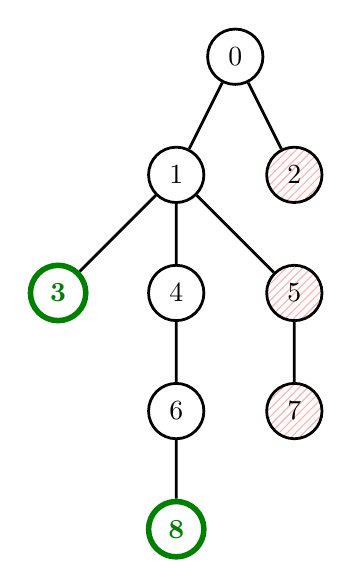
\begin{tikzpicture}[every node/.style={minimum width=2em,draw,circle,line width=1pt},
        edge from parent/.style=
        {draw,line width=1pt,edge from parent path={(\tikzparentnode) -- (\tikzchildnode)}},
        level distance=1.5cm,
        sibling distance=1.5cm,
        green/.style={color=green!50!black,line width=2pt,font=\bf},
        marked/.style={pattern=north east lines,pattern color=red!30}]

    \node {0}
    child {
        node {1}
        child {
            node[green] {3}
        }
        child {
            node {4}
            child {
                node {6}
                child {
                    node[green] {8}
                }
            }
        }
        child[marked] {
            node[marked] {5}
            child[marked] {
                node[marked] {7}
            }
        }
    }
    child[marked] {
        node[marked] {2}
    };
\end{tikzpicture}
\end{document}
